\documentclass[Ligatures=TeX,table,brazil,svgnames,usetotalslideindicator,compress,10pt]{beamer}

\usetheme[titleformat=allsmallcaps]{metropolis}

\usepackage{polyglossia}
\setdefaultlanguage{brazil}
\disablehyphenation

\usepackage{minted}

\usetikzlibrary{arrows,positioning,calc}

\usepackage{graphicx}
\graphicspath{{./figuras/}}
\usepackage{subcaption}
\usepackage{xmpmulti}

%\usepackage{textpos}

%\usepackage{mdwlist}
%\usepackage{siunitx}
\usepackage{alltt}
%\usepackage{multicol}
\usepackage{xspace}
\usepackage{multirow}
\usepackage{amsmath}

\usepackage{cancel}


\newcommand{\setcoverbg}{
    \setbeamertemplate{background}
     {
\includegraphics[width=\paperwidth,height=\paperheight]{backgrounds/coverbg}}
}
\newcommand{\setintersectionbg}{
    \setbeamertemplate{background}
     {
\includegraphics[width=\paperwidth,height=\paperheight]{backgrounds/blank}}
}
\newcommand{\setsectionbg}{
    \setbeamertemplate{background}
     {
\includegraphics[width=\paperwidth,height=\paperheight]{backgrounds/slidebg2}}
}

\setbeamertemplate{caption}{default}

\title{MCTA025-13 - Sistemas Distribuídos}
\subtitle{Tipos de Sistemas Distribuídos}

\author{Emilio Francesquini}
\institute{Centro de Matemática, Computação e Cognição\\ Universidade Federal do ABC}
\date{11 de junho de 2018}

\begin{document}

\setcoverbg
\maketitle

\setsectionbg

\begin{frame}
  \frametitle{Disclaimer}
  \begin{itemize}
  \item Estes slides foram preparados para o curso de \textbf{Sistemas
      Distribuídos na UFABC}.
  \item Este material pode ser usado livremente desde que sejam
    mantidos, além deste aviso, os créditos aos autores e
    instituições.
  \item Estes slides foram adaptados daqueles originalmente preparados
    (e gentilmente cedidos) pelo professor \textbf{Daniel Cordeiro, da
      EACH-USP} que por sua vez foram baseados naqueles
    disponibilizados online pelos autores do livro ``Distributed
    Systems'', 3ª Edição em:
    \url{https://www.distributed-systems.net}.

  \end{itemize}
\end{frame}

\begin{frame}
  \frametitle{Três tipos de sistemas distribuídos}
  \begin{itemize}
  \item Sistemas para computação distribuída de alto desempenho
  \item Sistemas de informação distribuídos
  \item Sistemas distribuídos para computação ubíqua
  \end{itemize}
\end{frame}

\begin{frame}
  \frametitle{Computação paralela}
  \begin{block}{Observação}
    A computação distribuída de alto desempenho  foi originada na computação paralela
  \end{block}

  \begin{block}{Multiprocessadores e multicores versus multicomputadores}
    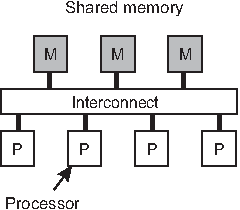
\includegraphics{01-06a}
    \quad \vrule{} \quad
    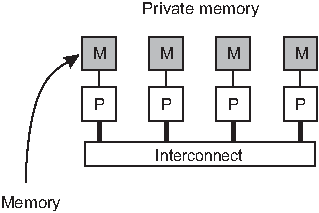
\includegraphics{01-06b}
  \end{block}
\end{frame}

\begin{frame}
  \frametitle{Sistemas de memória  compartilhada distribuída}
  \small
  \begin{block}{Observação}
    Multiprocessadores são relativamente fáceis de programar se comparados a multicomputadores, mas ainda assim os problemas aparecem quando o número de processadores (ou cores) aumentam. Solução: tentar implementar um modelo de memória compartilhada para multicomputadores.
  \end{block}

  \begin{exampleblock}{Exemplo usando técnicas de memória virtual}
    Mapear todas as páginas da memória principal (de todos os diferentes processadores) em um único espaço de endereçamento virtual. Se o processo no processador $A$ referenciar uma página $P$ localizada no processador $B$, o SO em $A$ lança uma interrupção e recupera $P$ de $B$, do mesmo modo que faria se $P$ estivesse localizado no disco.
\end{exampleblock}

\begin{block}{Problema}
  O desempenho de um sistema de memória compartilhada distribuída nunca poderia competir com o desempenho de multiprocessadores e, por isso, a ideia foi abandonada por enquanto.
\end{block}

\end{frame}

\begin{frame}
  \frametitle{Aglomerados de computação (cluster computing)}
  \begin{block}{Essencialmente um grupo de computadores de boa qualidade conectados via LAN}

    \begin{itemize}
    \item Homogêneo: mesmo SO, hardware quase idêntico
    \item Um único nó gerenciador
    \end{itemize}
  \end{block}

  \begin{figure}
    \centering
    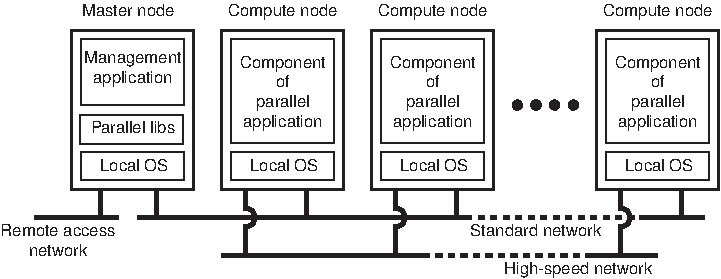
\includegraphics[width=\textwidth]{01-06}
  \end{figure}
\end{frame}

\begin{frame}
  \frametitle{Computação em Grade}


  \begin{block}{O próximo passo: vários nós vindos de todos os cantos:}
  \begin{itemize}
  \item Heterogêneos
  \item Espalhados entre diversas organizações
  \item Normalmente formam uma rede de longa distância (\textit{wide-area network})
  \end{itemize}
\end{block}

  \begin{alertblock}{Nota:}
    Para permitir colaborações, grades normalmente usam
    \emph{organizações virtuais}. Essencialmente, isso significa que
    os usuários (ou melhor, seus IDs) são organizados em grupos que
    possuem autorização para usar alguns recursos.
  \end{alertblock}

\end{frame}

\begin{frame}
  \frametitle{Arquitetura de computação em grade}
  \begin{columns}
    \begin{column}{0.4\textwidth}
      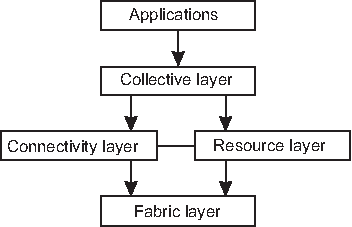
\includegraphics[scale=1]{01-08}
    \end{column}
    \quad
    \small
        \begin{column}{0.6\textwidth}
          \begin{block}{Camadas}
            \begin{description}
            \item[Infraestrutura] provê interfaces para os recursos locais
            \item[Conectividade] protocolos de comunicação/transação e autenticação
            \item[Recurso] gerencia um único recurso, por exemplo criando processos ou lendo dados
            \item[Coletiva] realiza acesso à múltiplos recursos: descoberta, escalonamento, replicação
            \item[Aplicação] contém a aplicação real da grade em uma única organização
            \end{description}
          \end{block}
    \end{column}
  \end{columns}
\end{frame}


\begin{frame}
  \frametitle{Sistemas de Computação Distribuídos: Computação em Nuvem}
  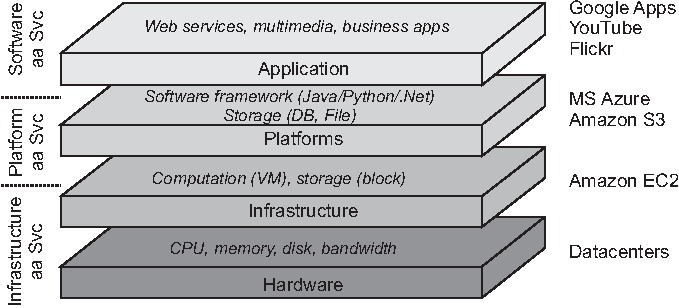
\includegraphics{01-cloud}
\end{frame}

\begin{frame}
  \frametitle{Sistemas de Computação Distribuídos: Computação em Nuvem}

  \begin{block}{Computação em nuvem}
    Faz uma distinção entre quatro camadas:

    \begin{description}
    \item[Hardware] processadores, roteadores, energia, sistemas de refrigeração
    \item[Infraestrutura] Utiliza técnicas de virtualização para alocação e gerenciamento de armazenamento e servidores virtuais
    \item[Plataforma] Provê abstrações de alto nível para os serviços da plataforma. Ex: Amazon S3 para armazenamento de arquivos em \textit{buckets}
    \item[Aplicação] as aplicações propriamente ditas, tais como as suítes de aplicativos para escritórios.
    \end{description}

  \end{block}

\end{frame}

\begin{frame}
  \frametitle{Usar computação em nuvem é economicamente viável?}
  \begin{block}{Observação}
    Uma razão importante para o sucesso de computação em nuvem é que ela permite que organizações terceirizem sua infraestrutura de TI: hardware e software. A pergunta é: terceirizar é mesmo mais barato?
  \end{block}

  \begin{block}{Abordagem}
    \begin{itemize}
    \item Considere \emph{aplicações corporativas}, modeladas como uma coleção de componentes ($C_i$), cada qual precisando de $N_i$ servidores
    \item Podemos ver a aplicação como um \alert{grafo dirigido}, com um vértice representando um componente e um arco $\vec{\langle i,j \rangle}$ representando o fluxo de dados de $C_i$ para $C_j$.
    \item Cada arco tem dois pesos associados:
      \begin{itemize}
      \item $T_{i,j}$, o número de transações por unidade de tempo que causam o fluxo de dados de $C_i$ para $C_j$
      \item $S_{i,j}$, a quantidade de dados total associada a $T_{i,j}$
      \end{itemize}
    \end{itemize}
  \end{block}
\end{frame}

\begin{frame}
  \frametitle{Usar computação em nuvem é economicamente viável?}
  \begin{block}{Plano de migração}
    Encontre para cada componente $C_i$, quantos dos $n_i$ dentre seus $N_i$ servidores deveriam migrar, tal que a economia no orçamento menos os cursos de comunicação via Internet sejam maximais.
  \end{block}
  \begin{block}{Requisitos para o plano de migração}
    \begin{enumerate}
    \item As restrições impostas pelas políticas devem ser respeitadas
    \item Latências adicionais não violarão nenhuma das restrições
    \item Todas as transações continuarão a operar corretamente; requisições ou dados não serão perdidos durante a transação
    \end{enumerate}
  \end{block}
\end{frame}

\begin{frame}
  \frametitle{Calculando os benefícios}
  \begin{block}{Economia no orçamento}
    \begin{itemize}
    \item $B_c$: economias com a migração de um componente computacionalmente intensivo
    \item $M_c$ número total de componentes computacionalmente intensivos
    \item $B_s$: economias com a migração de um componente intensivo em armazenamento
    \item $M_s$ número total de componentes  intensivos em armazenamento
    \end{itemize}
    A economia total, obviamente, é: $B_c \times M_c + B_s \times M_s$.
  \end{block}
\end{frame}

\begin{frame}
  \frametitle{Custos com Internet}
  \begin{block}{Tráfego de/para a nuvem}
    \[Tr_{\text{local, inet}} = \sum_{C_i}
       ( T_{\text{usuário},i}S_{\text{usuário},i} + T_{i,\text{usuário}}S_{i,\text{usuário}} )\]
  \end{block}

    \begin{itemize}
    \item $T_{\text{usuário},i}$: transações por unidade de tempo que causam fluxo de dados do usuário para $C_i$
    \item $S_{\text{usuário},i}$ quantidade de dados associados com $T_{\text{usuário},i}$
    \end{itemize}
\end{frame}

\begin{frame}
  \frametitle{Taxa de transações após migração}
  \begin{block}{Mais notações:}
    \begin{itemize}
    \item $C_{i,\text{local}}$: conjunto de servidores de $C_i$ que continuam executando localmente
    \item $C_{i,\text{cloud}}$: conjunto de servidores de $C_i$ migrados para o cloud
    \item Assuma que a distribuição de tráfego é a mesma para o servidor local ou no cloud.
    \end{itemize}
    Note que $|C_{i,\text{cloud}} = n_i|$. Seja $f_i = n_i/N_i$ e $s_i$ um servidor de $C_i$.
  \end{block}

      \begin{block}{}
      \[ T^*_{i,j} = 
      \begin{cases}
        (1-f_i) \cdot (1-f_j) \cdot T_{i,j} & \text{quando } s_i \in C_{i,local} \text{ e } s_j \in C_{j,local} \\
        (1-f_i) \cdot f_j \cdot T_{i,j} & \text{quando } s_i \in C_{i,local} \text{ e } s_j \in C_{j,cloud} \\
        f_i \cdot (1-f_j) \cdot T_{i,j} & \text{quando } s_i \in C_{i,cloud} \text{ e } s_j \in C_{j,local} \\
        f_i \cdot f_j \cdot T_{i,j} & \text{quando } s_i \in C_{i,cloud} \text{ e } s_j \in C_{j,cloud} \\
      \end{cases}
      \]
    \end{block}
\end{frame}



\begin{frame}[fragile]
  \frametitle{Sistemas de Informação Distribuídos}
  \begin{block}{Observação:}
    Uma quantidade enorme de sistemas distribuídos em uso hoje em dia são formas de sistemas de informação tradicionais, \emph{integrando} sistemas legados. \alert{Exemplo:} sistemas de processamento de transações.
  \end{block}

  {\scriptsize
  \begin{verbatim}
    BEGIN_TRANSACTION(server, transaction)
    READ(transaction, file-1, data)
    WRITE(transaction, file-2, data)
    newData := MODIFIED(data)
    IF WRONG(newData) THEN  
        ABORT_TRANSACTION(transaction)
    ELSE   
        WRITE(transaction, file-2, newData) 
        END_TRANSACTION(transaction)
    END IF 
  \end{verbatim}}
  
  \onslide<2->
  \begin{alertblock}{Nota:}
    Transações formam uma operação \alert{atômica}.
  \end{alertblock}

\end{frame}

\begin{frame}
  \frametitle{Sistemas de Informação Distribuídos: Transações}

  Uma transação é um conjunto de operações sobre o estado de um objeto (banco de dados, composição de objetos, etc.) que satisfazem as seguintes propriedades (\alert{ACID}):

  \begin{description}[<+->]
  \item[Atomicidade] ou todas as operações são bem sucedidas, ou todas falham. Quando uma transação falha, o estado do objeto permanecerá inalterado.
  \item[Consistência] uma transação estabelece um estado de transição válido. Isto não exclui a existência de estados intermediários inválidos durante sua execução.
  \item[Isolamento] transações concorrentes não interferem entre
    si. Para uma transação $T$ é como se as outras transações
    ocorressem ou \emph{antes} de $T$, ou \emph{depois} de $T$.
  \item[Durabilidade] Após o término de uma transação, seus efeitos são permanentes: mudanças de estado sobrevivem a falhas.
  \end{description}
  
\end{frame}

\begin{frame}
  \frametitle{Monitor de Processamento de Transações}
  
  \begin{block}{Observação:}
    Em muitos casos, o conjunto de dados envolvidos em uma transação está distribuído em vários servidores. Um \alert{TP Monitor} é responsável por coordenar a execução de uma transação.
  \end{block}

  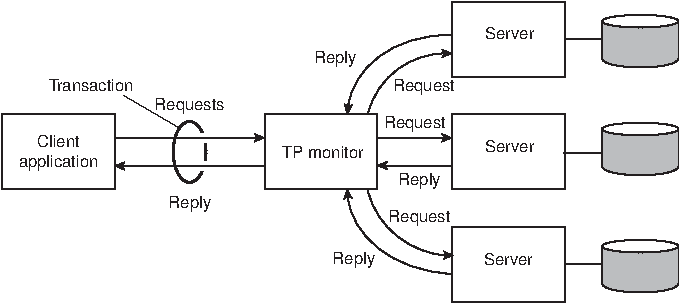
\includegraphics[scale=0.83]{01-10}

\end{frame}

\begin{frame}
  \frametitle{S.I. Distribuídas.: Integração de Aplicações Corporativas}

  \begin{block}{Problema}
    Um TP Monitor não basta, também são necessários mecanismos para a comunicação direta entre aplicações.
  \end{block}
 
  \begin{figure}
    \centering
    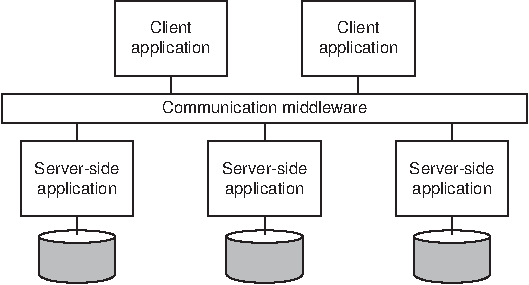
\includegraphics[scale=0.83]{01-11}
  \end{figure}
  
  \begin{itemize}
  \item \alert{Chamada de Procedimento Remoto} (RPC)
  \item \alert{Middleware Orientado a Mensagens} (MOM)
  \end{itemize}

\end{frame}

\begin{frame}
  \frametitle{Sistemas Distribuídos Ubíquos}

    Tendência em sistemas distribuídos; nós são pequenos, móveis e
    normalmente embutidos em um sistema muito maior.


  \begin{block}{Alguns requisitos:}
    \begin{itemize}
    \item \alert{Mudança contextual}: o sistema é parte de um ambiente onde mudanças devem ser rapidamente levadas em consideração
    \item \alert{Composição ad hoc}:  cada nó pode ser usado em diferentes maneiras, por diferentes usuários. Deve ser facilmente configurável.
    \item \alert{Compartilhar é o padrão}: nós vão e vêm, fornecendo serviços e informação compartilháveis. Pede simplicidade.
    \end{itemize}
  \end{block}

  \pause
  \begin{alertblock}{Nota:}
    Ubiquidade e transparência de distribuição formam um bom par?
  \end{alertblock}

\end{frame}

\begin{frame}
  \frametitle{Sistemas Ubíquos: exemplos}
  \begin{block}{Sistemas domésticos}
    Devem ser completamente auto-organizáveis:
    \begin{itemize}
    \item Não deve haver um administrador do sistema
    \item Solução mais simples: um \alert{home box} centralizado?
    \end{itemize}
  \end{block}

  \pause
  \begin{block}{Monitorando uma pessoa}
    Dispositivos ficam fisicamente próximos a uma pessoa:
    \begin{itemize}
    \item Onde e como são armazenados os dados monitorados?
    \item Podemos prevenir perda de dados importantes?
    \item Há necessidade de gerar e propagar alertas?
    \item Como fazer para garantir segurança?
    \item Como o ambiente pode prover \textit{feedback} online?
    \end{itemize}
  \end{block}
\end{frame}

\begin{frame}
  \frametitle{Redes de sensores}
  \begin{block}{Características}
    Os nós aos quais os sensores estão presos são:
    \begin{itemize}
    \item Muitos (10s--1000s)
    \item Simples (pouca capacidade de memória/computação/comunicação)
    \item Normalmente necessitam de uma bateria
    \end{itemize}
  \end{block}
\end{frame}

\begin{frame}
  \frametitle{Redes de sensores como um sistema distribuído}
  \begin{center}
    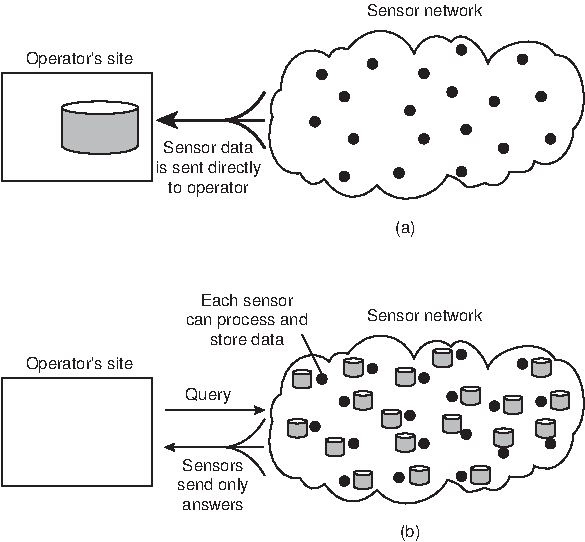
\includegraphics[scale=0.83]{01-13}
  \end{center}
\end{frame}

\begin{frame}
  \frametitle{Possíveis exemplos}
  
  \begin{block}{Gerenciamento de multidões}
    \begin{itemize}
    \item \alert{Situação:} um grande evento sem rotas fixas (exposições, festivais, etc.)
    \item \alert{Objetivo:} guiar as pessoas de acordo com suas posições sociais:
      \begin{itemize}
      \item direcionar pessoas com interesses similares para os mesmos locais
      \item direcionar membros de um grupo para uma mesma saída no caso de uma emergência 
      \end{itemize}
    \item \alert{Objetivo:} manter grupos unidos (p.ex.:, famílias)
    \end{itemize}
  \end{block}

  \vspace{-1em}
  \begin{center}
    \begin{tabular}{cc}
      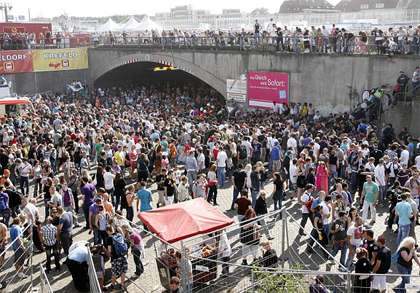
\includegraphics[width=0.35\textwidth]{love2010.jpg} &
      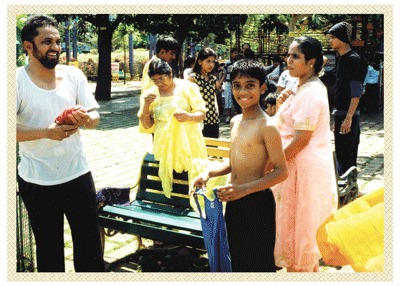
\includegraphics[width=0.35\textwidth]{family.jpg} 
    \end{tabular}
  \end{center}

\end{frame}

\begin{frame}
  \frametitle{Cenários de aplicação: jogos sociais}
  \begin{block}{Estimulando a mistura}
    \begin{itemize}
    \item \alert{Situação:} conferência com pessoas de diferentes grupos
    \item \alert{Objetivo:} estimular pessoas de diferentes grupos a interagirem.
    \item \alert{Abordagem:} acompanhar as interações entre os grupos:
    \begin{itemize}
    \item Quando um aluno de BC\&T fala com um aluno de BC\&H: pontos de bônus para os dois alunos e para os seus respectivos grupos.
    \item Pontos para o grupo são distribuídos entre os seus membros
    \item Conquistas são mostradas em crachás eletrônicos (\emph{feedback} e \emph{intervenções sociais})
    \end{itemize}
    \end{itemize}
  \end{block}
\end{frame}

\begin{frame}
  \frametitle{Cenários de aplicação: jogos sociais}

  \begin{center}
    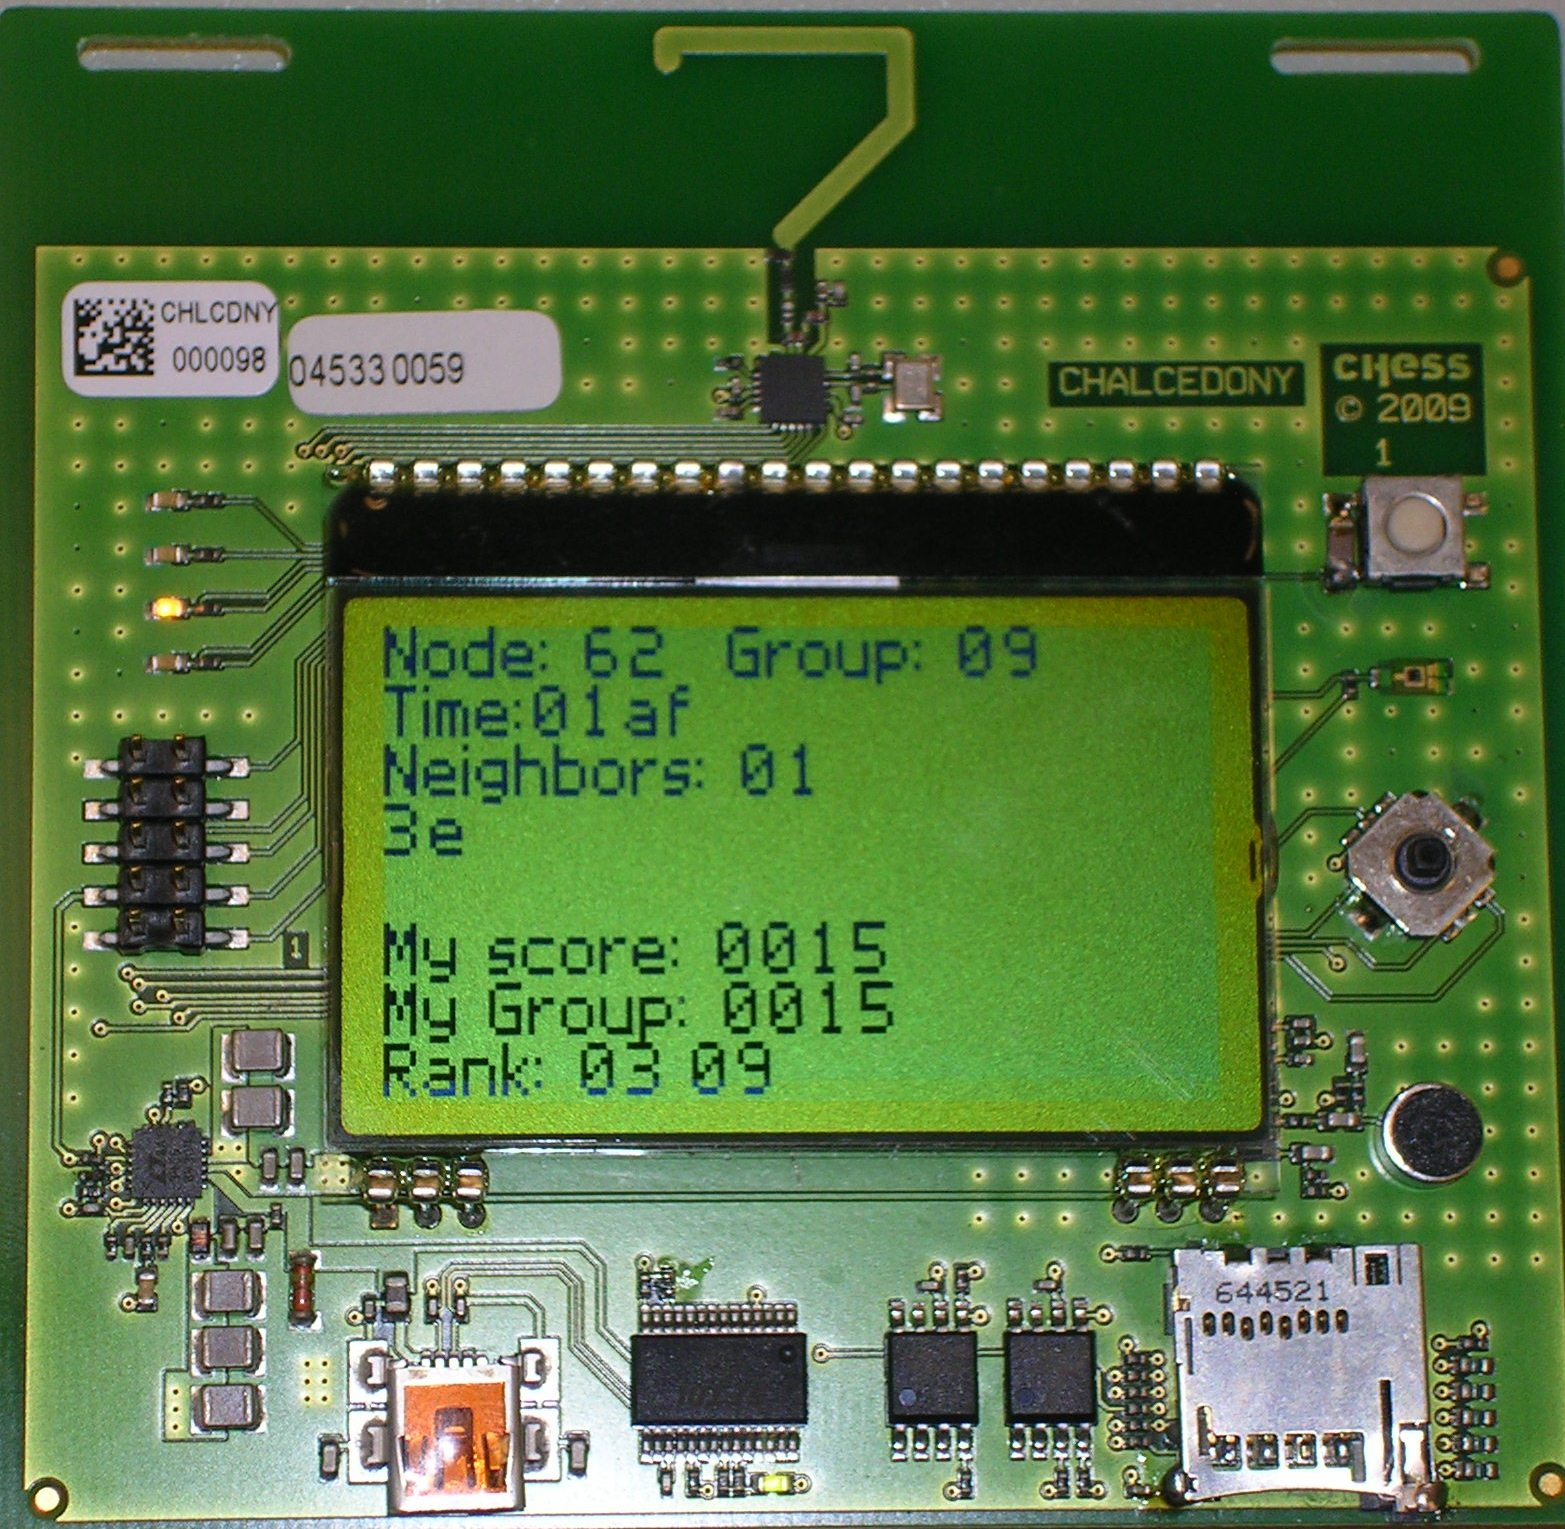
\includegraphics[width=0.75\textheight]{chalcedony.jpg}
  \end{center}
\end{frame}  

% \begin{frame}[fragile]
%   \frametitle{Diferentes tipos de sistemas distribuídos}

%   \only<1>{
%   \begin{figure}
%     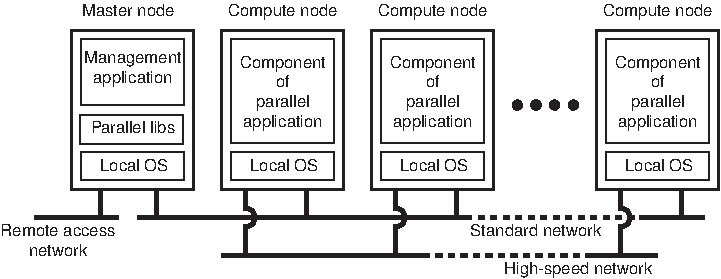
\includegraphics[scale=0.83]{01-06}
%     \caption{Aglomerados}
%   \end{figure}}

%   \only<2>{
%     \begin{figure}
%       \begin{subfigure}{0.43\textwidth}
%         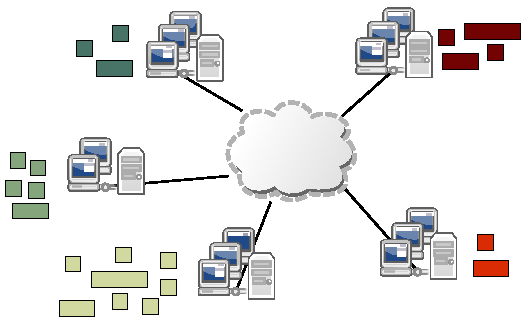
\includegraphics[width=\textwidth]{grid-computing-1}
%       \end{subfigure}
%       \quad \vrule \quad
%       \begin{subfigure}{0.43\textwidth}
%         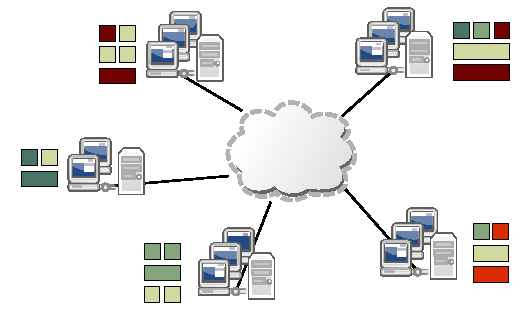
\includegraphics[width=\textwidth]{grid-computing-2}
%       \end{subfigure}
%       \caption{Computação em Grades}
%     \end{figure}
%   }

%   \only<3>{
%     \begin{figure}
%       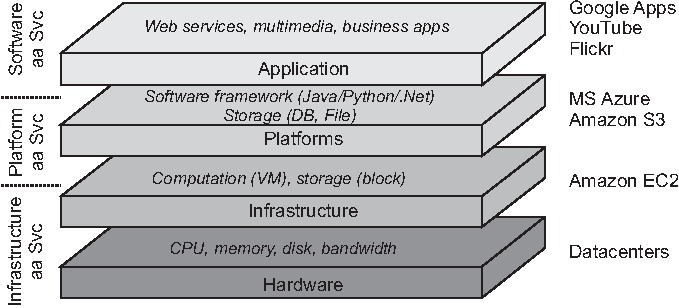
\includegraphics{01-cloud}
%       \caption{Computação em Nuvem}
%     \end{figure}
%   }

% \end{frame}

\end{document}
